\documentclass[11pt]{article}

    \usepackage[breakable]{tcolorbox}
    \usepackage{parskip} % Stop auto-indenting (to mimic markdown behaviour)
    
    \usepackage{iftex}
    \ifPDFTeX
    	\usepackage[T1]{fontenc}
    	\usepackage{mathpazo}
    \else
    	\usepackage{fontspec}
    \fi

    % Basic figure setup, for now with no caption control since it's done
    % automatically by Pandoc (which extracts ![](path) syntax from Markdown).
    \usepackage{graphicx}
    % Maintain compatibility with old templates. Remove in nbconvert 6.0
    \let\Oldincludegraphics\includegraphics
    % Ensure that by default, figures have no caption (until we provide a
    % proper Figure object with a Caption API and a way to capture that
    % in the conversion process - todo).
    \usepackage{caption}
    \DeclareCaptionFormat{nocaption}{}
    \captionsetup{format=nocaption,aboveskip=0pt,belowskip=0pt}

    \usepackage[Export]{adjustbox} % Used to constrain images to a maximum size
    \adjustboxset{max size={0.9\linewidth}{0.9\paperheight}}
    \usepackage{float}
    \floatplacement{figure}{H} % forces figures to be placed at the correct location
    \usepackage{xcolor} % Allow colors to be defined
    \usepackage{enumerate} % Needed for markdown enumerations to work
    \usepackage{geometry} % Used to adjust the document margins
    \usepackage{amsmath} % Equations
    \usepackage{amssymb} % Equations
    \usepackage{textcomp} % defines textquotesingle
    % Hack from http://tex.stackexchange.com/a/47451/13684:
    \AtBeginDocument{%
        \def\PYZsq{\textquotesingle}% Upright quotes in Pygmentized code
    }
    \usepackage{upquote} % Upright quotes for verbatim code
    \usepackage{eurosym} % defines \euro
    \usepackage[mathletters]{ucs} % Extended unicode (utf-8) support
    \usepackage{fancyvrb} % verbatim replacement that allows latex
    \usepackage{grffile} % extends the file name processing of package graphics 
                         % to support a larger range
    \makeatletter % fix for grffile with XeLaTeX
    \def\Gread@@xetex#1{%
      \IfFileExists{"\Gin@base".bb}%
      {\Gread@eps{\Gin@base.bb}}%
      {\Gread@@xetex@aux#1}%
    }
    \makeatother

    % The hyperref package gives us a pdf with properly built
    % internal navigation ('pdf bookmarks' for the table of contents,
    % internal cross-reference links, web links for URLs, etc.)
    \usepackage{hyperref}
    % The default LaTeX title has an obnoxious amount of whitespace. By default,
    % titling removes some of it. It also provides customization options.
    \usepackage{titling}
    \usepackage{longtable} % longtable support required by pandoc >1.10
    \usepackage{booktabs}  % table support for pandoc > 1.12.2
    \usepackage[inline]{enumitem} % IRkernel/repr support (it uses the enumerate* environment)
    \usepackage[normalem]{ulem} % ulem is needed to support strikethroughs (\sout)
                                % normalem makes italics be italics, not underlines
    \usepackage{mathrsfs}
    

    
    % Colors for the hyperref package
    \definecolor{urlcolor}{rgb}{0,.145,.698}
    \definecolor{linkcolor}{rgb}{.71,0.21,0.01}
    \definecolor{citecolor}{rgb}{.12,.54,.11}

    % ANSI colors
    \definecolor{ansi-black}{HTML}{3E424D}
    \definecolor{ansi-black-intense}{HTML}{282C36}
    \definecolor{ansi-red}{HTML}{E75C58}
    \definecolor{ansi-red-intense}{HTML}{B22B31}
    \definecolor{ansi-green}{HTML}{00A250}
    \definecolor{ansi-green-intense}{HTML}{007427}
    \definecolor{ansi-yellow}{HTML}{DDB62B}
    \definecolor{ansi-yellow-intense}{HTML}{B27D12}
    \definecolor{ansi-blue}{HTML}{208FFB}
    \definecolor{ansi-blue-intense}{HTML}{0065CA}
    \definecolor{ansi-magenta}{HTML}{D160C4}
    \definecolor{ansi-magenta-intense}{HTML}{A03196}
    \definecolor{ansi-cyan}{HTML}{60C6C8}
    \definecolor{ansi-cyan-intense}{HTML}{258F8F}
    \definecolor{ansi-white}{HTML}{C5C1B4}
    \definecolor{ansi-white-intense}{HTML}{A1A6B2}
    \definecolor{ansi-default-inverse-fg}{HTML}{FFFFFF}
    \definecolor{ansi-default-inverse-bg}{HTML}{000000}

    % commands and environments needed by pandoc snippets
    % extracted from the output of `pandoc -s`
    \providecommand{\tightlist}{%
      \setlength{\itemsep}{0pt}\setlength{\parskip}{0pt}}
    \DefineVerbatimEnvironment{Highlighting}{Verbatim}{commandchars=\\\{\}}
    % Add ',fontsize=\small' for more characters per line
    \newenvironment{Shaded}{}{}
    \newcommand{\KeywordTok}[1]{\textcolor[rgb]{0.00,0.44,0.13}{\textbf{{#1}}}}
    \newcommand{\DataTypeTok}[1]{\textcolor[rgb]{0.56,0.13,0.00}{{#1}}}
    \newcommand{\DecValTok}[1]{\textcolor[rgb]{0.25,0.63,0.44}{{#1}}}
    \newcommand{\BaseNTok}[1]{\textcolor[rgb]{0.25,0.63,0.44}{{#1}}}
    \newcommand{\FloatTok}[1]{\textcolor[rgb]{0.25,0.63,0.44}{{#1}}}
    \newcommand{\CharTok}[1]{\textcolor[rgb]{0.25,0.44,0.63}{{#1}}}
    \newcommand{\StringTok}[1]{\textcolor[rgb]{0.25,0.44,0.63}{{#1}}}
    \newcommand{\CommentTok}[1]{\textcolor[rgb]{0.38,0.63,0.69}{\textit{{#1}}}}
    \newcommand{\OtherTok}[1]{\textcolor[rgb]{0.00,0.44,0.13}{{#1}}}
    \newcommand{\AlertTok}[1]{\textcolor[rgb]{1.00,0.00,0.00}{\textbf{{#1}}}}
    \newcommand{\FunctionTok}[1]{\textcolor[rgb]{0.02,0.16,0.49}{{#1}}}
    \newcommand{\RegionMarkerTok}[1]{{#1}}
    \newcommand{\ErrorTok}[1]{\textcolor[rgb]{1.00,0.00,0.00}{\textbf{{#1}}}}
    \newcommand{\NormalTok}[1]{{#1}}
    
    % Additional commands for more recent versions of Pandoc
    \newcommand{\ConstantTok}[1]{\textcolor[rgb]{0.53,0.00,0.00}{{#1}}}
    \newcommand{\SpecialCharTok}[1]{\textcolor[rgb]{0.25,0.44,0.63}{{#1}}}
    \newcommand{\VerbatimStringTok}[1]{\textcolor[rgb]{0.25,0.44,0.63}{{#1}}}
    \newcommand{\SpecialStringTok}[1]{\textcolor[rgb]{0.73,0.40,0.53}{{#1}}}
    \newcommand{\ImportTok}[1]{{#1}}
    \newcommand{\DocumentationTok}[1]{\textcolor[rgb]{0.73,0.13,0.13}{\textit{{#1}}}}
    \newcommand{\AnnotationTok}[1]{\textcolor[rgb]{0.38,0.63,0.69}{\textbf{\textit{{#1}}}}}
    \newcommand{\CommentVarTok}[1]{\textcolor[rgb]{0.38,0.63,0.69}{\textbf{\textit{{#1}}}}}
    \newcommand{\VariableTok}[1]{\textcolor[rgb]{0.10,0.09,0.49}{{#1}}}
    \newcommand{\ControlFlowTok}[1]{\textcolor[rgb]{0.00,0.44,0.13}{\textbf{{#1}}}}
    \newcommand{\OperatorTok}[1]{\textcolor[rgb]{0.40,0.40,0.40}{{#1}}}
    \newcommand{\BuiltInTok}[1]{{#1}}
    \newcommand{\ExtensionTok}[1]{{#1}}
    \newcommand{\PreprocessorTok}[1]{\textcolor[rgb]{0.74,0.48,0.00}{{#1}}}
    \newcommand{\AttributeTok}[1]{\textcolor[rgb]{0.49,0.56,0.16}{{#1}}}
    \newcommand{\InformationTok}[1]{\textcolor[rgb]{0.38,0.63,0.69}{\textbf{\textit{{#1}}}}}
    \newcommand{\WarningTok}[1]{\textcolor[rgb]{0.38,0.63,0.69}{\textbf{\textit{{#1}}}}}
    
    
    % Define a nice break command that doesn't care if a line doesn't already
    % exist.
    \def\br{\hspace*{\fill} \\* }
    % Math Jax compatibility definitions
    \def\gt{>}
    \def\lt{<}
    \let\Oldtex\TeX
    \let\Oldlatex\LaTeX
    \renewcommand{\TeX}{\textrm{\Oldtex}}
    \renewcommand{\LaTeX}{\textrm{\Oldlatex}}
    % Document parameters
    % Document title
    \title{README}
    
    
    
    
    
% Pygments definitions
\makeatletter
\def\PY@reset{\let\PY@it=\relax \let\PY@bf=\relax%
    \let\PY@ul=\relax \let\PY@tc=\relax%
    \let\PY@bc=\relax \let\PY@ff=\relax}
\def\PY@tok#1{\csname PY@tok@#1\endcsname}
\def\PY@toks#1+{\ifx\relax#1\empty\else%
    \PY@tok{#1}\expandafter\PY@toks\fi}
\def\PY@do#1{\PY@bc{\PY@tc{\PY@ul{%
    \PY@it{\PY@bf{\PY@ff{#1}}}}}}}
\def\PY#1#2{\PY@reset\PY@toks#1+\relax+\PY@do{#2}}

\expandafter\def\csname PY@tok@w\endcsname{\def\PY@tc##1{\textcolor[rgb]{0.73,0.73,0.73}{##1}}}
\expandafter\def\csname PY@tok@c\endcsname{\let\PY@it=\textit\def\PY@tc##1{\textcolor[rgb]{0.25,0.50,0.50}{##1}}}
\expandafter\def\csname PY@tok@cp\endcsname{\def\PY@tc##1{\textcolor[rgb]{0.74,0.48,0.00}{##1}}}
\expandafter\def\csname PY@tok@k\endcsname{\let\PY@bf=\textbf\def\PY@tc##1{\textcolor[rgb]{0.00,0.50,0.00}{##1}}}
\expandafter\def\csname PY@tok@kp\endcsname{\def\PY@tc##1{\textcolor[rgb]{0.00,0.50,0.00}{##1}}}
\expandafter\def\csname PY@tok@kt\endcsname{\def\PY@tc##1{\textcolor[rgb]{0.69,0.00,0.25}{##1}}}
\expandafter\def\csname PY@tok@o\endcsname{\def\PY@tc##1{\textcolor[rgb]{0.40,0.40,0.40}{##1}}}
\expandafter\def\csname PY@tok@ow\endcsname{\let\PY@bf=\textbf\def\PY@tc##1{\textcolor[rgb]{0.67,0.13,1.00}{##1}}}
\expandafter\def\csname PY@tok@nb\endcsname{\def\PY@tc##1{\textcolor[rgb]{0.00,0.50,0.00}{##1}}}
\expandafter\def\csname PY@tok@nf\endcsname{\def\PY@tc##1{\textcolor[rgb]{0.00,0.00,1.00}{##1}}}
\expandafter\def\csname PY@tok@nc\endcsname{\let\PY@bf=\textbf\def\PY@tc##1{\textcolor[rgb]{0.00,0.00,1.00}{##1}}}
\expandafter\def\csname PY@tok@nn\endcsname{\let\PY@bf=\textbf\def\PY@tc##1{\textcolor[rgb]{0.00,0.00,1.00}{##1}}}
\expandafter\def\csname PY@tok@ne\endcsname{\let\PY@bf=\textbf\def\PY@tc##1{\textcolor[rgb]{0.82,0.25,0.23}{##1}}}
\expandafter\def\csname PY@tok@nv\endcsname{\def\PY@tc##1{\textcolor[rgb]{0.10,0.09,0.49}{##1}}}
\expandafter\def\csname PY@tok@no\endcsname{\def\PY@tc##1{\textcolor[rgb]{0.53,0.00,0.00}{##1}}}
\expandafter\def\csname PY@tok@nl\endcsname{\def\PY@tc##1{\textcolor[rgb]{0.63,0.63,0.00}{##1}}}
\expandafter\def\csname PY@tok@ni\endcsname{\let\PY@bf=\textbf\def\PY@tc##1{\textcolor[rgb]{0.60,0.60,0.60}{##1}}}
\expandafter\def\csname PY@tok@na\endcsname{\def\PY@tc##1{\textcolor[rgb]{0.49,0.56,0.16}{##1}}}
\expandafter\def\csname PY@tok@nt\endcsname{\let\PY@bf=\textbf\def\PY@tc##1{\textcolor[rgb]{0.00,0.50,0.00}{##1}}}
\expandafter\def\csname PY@tok@nd\endcsname{\def\PY@tc##1{\textcolor[rgb]{0.67,0.13,1.00}{##1}}}
\expandafter\def\csname PY@tok@s\endcsname{\def\PY@tc##1{\textcolor[rgb]{0.73,0.13,0.13}{##1}}}
\expandafter\def\csname PY@tok@sd\endcsname{\let\PY@it=\textit\def\PY@tc##1{\textcolor[rgb]{0.73,0.13,0.13}{##1}}}
\expandafter\def\csname PY@tok@si\endcsname{\let\PY@bf=\textbf\def\PY@tc##1{\textcolor[rgb]{0.73,0.40,0.53}{##1}}}
\expandafter\def\csname PY@tok@se\endcsname{\let\PY@bf=\textbf\def\PY@tc##1{\textcolor[rgb]{0.73,0.40,0.13}{##1}}}
\expandafter\def\csname PY@tok@sr\endcsname{\def\PY@tc##1{\textcolor[rgb]{0.73,0.40,0.53}{##1}}}
\expandafter\def\csname PY@tok@ss\endcsname{\def\PY@tc##1{\textcolor[rgb]{0.10,0.09,0.49}{##1}}}
\expandafter\def\csname PY@tok@sx\endcsname{\def\PY@tc##1{\textcolor[rgb]{0.00,0.50,0.00}{##1}}}
\expandafter\def\csname PY@tok@m\endcsname{\def\PY@tc##1{\textcolor[rgb]{0.40,0.40,0.40}{##1}}}
\expandafter\def\csname PY@tok@gh\endcsname{\let\PY@bf=\textbf\def\PY@tc##1{\textcolor[rgb]{0.00,0.00,0.50}{##1}}}
\expandafter\def\csname PY@tok@gu\endcsname{\let\PY@bf=\textbf\def\PY@tc##1{\textcolor[rgb]{0.50,0.00,0.50}{##1}}}
\expandafter\def\csname PY@tok@gd\endcsname{\def\PY@tc##1{\textcolor[rgb]{0.63,0.00,0.00}{##1}}}
\expandafter\def\csname PY@tok@gi\endcsname{\def\PY@tc##1{\textcolor[rgb]{0.00,0.63,0.00}{##1}}}
\expandafter\def\csname PY@tok@gr\endcsname{\def\PY@tc##1{\textcolor[rgb]{1.00,0.00,0.00}{##1}}}
\expandafter\def\csname PY@tok@ge\endcsname{\let\PY@it=\textit}
\expandafter\def\csname PY@tok@gs\endcsname{\let\PY@bf=\textbf}
\expandafter\def\csname PY@tok@gp\endcsname{\let\PY@bf=\textbf\def\PY@tc##1{\textcolor[rgb]{0.00,0.00,0.50}{##1}}}
\expandafter\def\csname PY@tok@go\endcsname{\def\PY@tc##1{\textcolor[rgb]{0.53,0.53,0.53}{##1}}}
\expandafter\def\csname PY@tok@gt\endcsname{\def\PY@tc##1{\textcolor[rgb]{0.00,0.27,0.87}{##1}}}
\expandafter\def\csname PY@tok@err\endcsname{\def\PY@bc##1{\setlength{\fboxsep}{0pt}\fcolorbox[rgb]{1.00,0.00,0.00}{1,1,1}{\strut ##1}}}
\expandafter\def\csname PY@tok@kc\endcsname{\let\PY@bf=\textbf\def\PY@tc##1{\textcolor[rgb]{0.00,0.50,0.00}{##1}}}
\expandafter\def\csname PY@tok@kd\endcsname{\let\PY@bf=\textbf\def\PY@tc##1{\textcolor[rgb]{0.00,0.50,0.00}{##1}}}
\expandafter\def\csname PY@tok@kn\endcsname{\let\PY@bf=\textbf\def\PY@tc##1{\textcolor[rgb]{0.00,0.50,0.00}{##1}}}
\expandafter\def\csname PY@tok@kr\endcsname{\let\PY@bf=\textbf\def\PY@tc##1{\textcolor[rgb]{0.00,0.50,0.00}{##1}}}
\expandafter\def\csname PY@tok@bp\endcsname{\def\PY@tc##1{\textcolor[rgb]{0.00,0.50,0.00}{##1}}}
\expandafter\def\csname PY@tok@fm\endcsname{\def\PY@tc##1{\textcolor[rgb]{0.00,0.00,1.00}{##1}}}
\expandafter\def\csname PY@tok@vc\endcsname{\def\PY@tc##1{\textcolor[rgb]{0.10,0.09,0.49}{##1}}}
\expandafter\def\csname PY@tok@vg\endcsname{\def\PY@tc##1{\textcolor[rgb]{0.10,0.09,0.49}{##1}}}
\expandafter\def\csname PY@tok@vi\endcsname{\def\PY@tc##1{\textcolor[rgb]{0.10,0.09,0.49}{##1}}}
\expandafter\def\csname PY@tok@vm\endcsname{\def\PY@tc##1{\textcolor[rgb]{0.10,0.09,0.49}{##1}}}
\expandafter\def\csname PY@tok@sa\endcsname{\def\PY@tc##1{\textcolor[rgb]{0.73,0.13,0.13}{##1}}}
\expandafter\def\csname PY@tok@sb\endcsname{\def\PY@tc##1{\textcolor[rgb]{0.73,0.13,0.13}{##1}}}
\expandafter\def\csname PY@tok@sc\endcsname{\def\PY@tc##1{\textcolor[rgb]{0.73,0.13,0.13}{##1}}}
\expandafter\def\csname PY@tok@dl\endcsname{\def\PY@tc##1{\textcolor[rgb]{0.73,0.13,0.13}{##1}}}
\expandafter\def\csname PY@tok@s2\endcsname{\def\PY@tc##1{\textcolor[rgb]{0.73,0.13,0.13}{##1}}}
\expandafter\def\csname PY@tok@sh\endcsname{\def\PY@tc##1{\textcolor[rgb]{0.73,0.13,0.13}{##1}}}
\expandafter\def\csname PY@tok@s1\endcsname{\def\PY@tc##1{\textcolor[rgb]{0.73,0.13,0.13}{##1}}}
\expandafter\def\csname PY@tok@mb\endcsname{\def\PY@tc##1{\textcolor[rgb]{0.40,0.40,0.40}{##1}}}
\expandafter\def\csname PY@tok@mf\endcsname{\def\PY@tc##1{\textcolor[rgb]{0.40,0.40,0.40}{##1}}}
\expandafter\def\csname PY@tok@mh\endcsname{\def\PY@tc##1{\textcolor[rgb]{0.40,0.40,0.40}{##1}}}
\expandafter\def\csname PY@tok@mi\endcsname{\def\PY@tc##1{\textcolor[rgb]{0.40,0.40,0.40}{##1}}}
\expandafter\def\csname PY@tok@il\endcsname{\def\PY@tc##1{\textcolor[rgb]{0.40,0.40,0.40}{##1}}}
\expandafter\def\csname PY@tok@mo\endcsname{\def\PY@tc##1{\textcolor[rgb]{0.40,0.40,0.40}{##1}}}
\expandafter\def\csname PY@tok@ch\endcsname{\let\PY@it=\textit\def\PY@tc##1{\textcolor[rgb]{0.25,0.50,0.50}{##1}}}
\expandafter\def\csname PY@tok@cm\endcsname{\let\PY@it=\textit\def\PY@tc##1{\textcolor[rgb]{0.25,0.50,0.50}{##1}}}
\expandafter\def\csname PY@tok@cpf\endcsname{\let\PY@it=\textit\def\PY@tc##1{\textcolor[rgb]{0.25,0.50,0.50}{##1}}}
\expandafter\def\csname PY@tok@c1\endcsname{\let\PY@it=\textit\def\PY@tc##1{\textcolor[rgb]{0.25,0.50,0.50}{##1}}}
\expandafter\def\csname PY@tok@cs\endcsname{\let\PY@it=\textit\def\PY@tc##1{\textcolor[rgb]{0.25,0.50,0.50}{##1}}}

\def\PYZbs{\char`\\}
\def\PYZus{\char`\_}
\def\PYZob{\char`\{}
\def\PYZcb{\char`\}}
\def\PYZca{\char`\^}
\def\PYZam{\char`\&}
\def\PYZlt{\char`\<}
\def\PYZgt{\char`\>}
\def\PYZsh{\char`\#}
\def\PYZpc{\char`\%}
\def\PYZdl{\char`\$}
\def\PYZhy{\char`\-}
\def\PYZsq{\char`\'}
\def\PYZdq{\char`\"}
\def\PYZti{\char`\~}
% for compatibility with earlier versions
\def\PYZat{@}
\def\PYZlb{[}
\def\PYZrb{]}
\makeatother


    % For linebreaks inside Verbatim environment from package fancyvrb. 
    \makeatletter
        \newbox\Wrappedcontinuationbox 
        \newbox\Wrappedvisiblespacebox 
        \newcommand*\Wrappedvisiblespace {\textcolor{red}{\textvisiblespace}} 
        \newcommand*\Wrappedcontinuationsymbol {\textcolor{red}{\llap{\tiny$\m@th\hookrightarrow$}}} 
        \newcommand*\Wrappedcontinuationindent {3ex } 
        \newcommand*\Wrappedafterbreak {\kern\Wrappedcontinuationindent\copy\Wrappedcontinuationbox} 
        % Take advantage of the already applied Pygments mark-up to insert 
        % potential linebreaks for TeX processing. 
        %        {, <, #, %, $, ' and ": go to next line. 
        %        _, }, ^, &, >, - and ~: stay at end of broken line. 
        % Use of \textquotesingle for straight quote. 
        \newcommand*\Wrappedbreaksatspecials {% 
            \def\PYGZus{\discretionary{\char`\_}{\Wrappedafterbreak}{\char`\_}}% 
            \def\PYGZob{\discretionary{}{\Wrappedafterbreak\char`\{}{\char`\{}}% 
            \def\PYGZcb{\discretionary{\char`\}}{\Wrappedafterbreak}{\char`\}}}% 
            \def\PYGZca{\discretionary{\char`\^}{\Wrappedafterbreak}{\char`\^}}% 
            \def\PYGZam{\discretionary{\char`\&}{\Wrappedafterbreak}{\char`\&}}% 
            \def\PYGZlt{\discretionary{}{\Wrappedafterbreak\char`\<}{\char`\<}}% 
            \def\PYGZgt{\discretionary{\char`\>}{\Wrappedafterbreak}{\char`\>}}% 
            \def\PYGZsh{\discretionary{}{\Wrappedafterbreak\char`\#}{\char`\#}}% 
            \def\PYGZpc{\discretionary{}{\Wrappedafterbreak\char`\%}{\char`\%}}% 
            \def\PYGZdl{\discretionary{}{\Wrappedafterbreak\char`\$}{\char`\$}}% 
            \def\PYGZhy{\discretionary{\char`\-}{\Wrappedafterbreak}{\char`\-}}% 
            \def\PYGZsq{\discretionary{}{\Wrappedafterbreak\textquotesingle}{\textquotesingle}}% 
            \def\PYGZdq{\discretionary{}{\Wrappedafterbreak\char`\"}{\char`\"}}% 
            \def\PYGZti{\discretionary{\char`\~}{\Wrappedafterbreak}{\char`\~}}% 
        } 
        % Some characters . , ; ? ! / are not pygmentized. 
        % This macro makes them "active" and they will insert potential linebreaks 
        \newcommand*\Wrappedbreaksatpunct {% 
            \lccode`\~`\.\lowercase{\def~}{\discretionary{\hbox{\char`\.}}{\Wrappedafterbreak}{\hbox{\char`\.}}}% 
            \lccode`\~`\,\lowercase{\def~}{\discretionary{\hbox{\char`\,}}{\Wrappedafterbreak}{\hbox{\char`\,}}}% 
            \lccode`\~`\;\lowercase{\def~}{\discretionary{\hbox{\char`\;}}{\Wrappedafterbreak}{\hbox{\char`\;}}}% 
            \lccode`\~`\:\lowercase{\def~}{\discretionary{\hbox{\char`\:}}{\Wrappedafterbreak}{\hbox{\char`\:}}}% 
            \lccode`\~`\?\lowercase{\def~}{\discretionary{\hbox{\char`\?}}{\Wrappedafterbreak}{\hbox{\char`\?}}}% 
            \lccode`\~`\!\lowercase{\def~}{\discretionary{\hbox{\char`\!}}{\Wrappedafterbreak}{\hbox{\char`\!}}}% 
            \lccode`\~`\/\lowercase{\def~}{\discretionary{\hbox{\char`\/}}{\Wrappedafterbreak}{\hbox{\char`\/}}}% 
            \catcode`\.\active
            \catcode`\,\active 
            \catcode`\;\active
            \catcode`\:\active
            \catcode`\?\active
            \catcode`\!\active
            \catcode`\/\active 
            \lccode`\~`\~ 	
        }
    \makeatother

    \let\OriginalVerbatim=\Verbatim
    \makeatletter
    \renewcommand{\Verbatim}[1][1]{%
        %\parskip\z@skip
        \sbox\Wrappedcontinuationbox {\Wrappedcontinuationsymbol}%
        \sbox\Wrappedvisiblespacebox {\FV@SetupFont\Wrappedvisiblespace}%
        \def\FancyVerbFormatLine ##1{\hsize\linewidth
            \vtop{\raggedright\hyphenpenalty\z@\exhyphenpenalty\z@
                \doublehyphendemerits\z@\finalhyphendemerits\z@
                \strut ##1\strut}%
        }%
        % If the linebreak is at a space, the latter will be displayed as visible
        % space at end of first line, and a continuation symbol starts next line.
        % Stretch/shrink are however usually zero for typewriter font.
        \def\FV@Space {%
            \nobreak\hskip\z@ plus\fontdimen3\font minus\fontdimen4\font
            \discretionary{\copy\Wrappedvisiblespacebox}{\Wrappedafterbreak}
            {\kern\fontdimen2\font}%
        }%
        
        % Allow breaks at special characters using \PYG... macros.
        \Wrappedbreaksatspecials
        % Breaks at punctuation characters . , ; ? ! and / need catcode=\active 	
        \OriginalVerbatim[#1,codes*=\Wrappedbreaksatpunct]%
    }
    \makeatother

    % Exact colors from NB
    \definecolor{incolor}{HTML}{303F9F}
    \definecolor{outcolor}{HTML}{D84315}
    \definecolor{cellborder}{HTML}{CFCFCF}
    \definecolor{cellbackground}{HTML}{F7F7F7}
    
    % prompt
    \makeatletter
    \newcommand{\boxspacing}{\kern\kvtcb@left@rule\kern\kvtcb@boxsep}
    \makeatother
    \newcommand{\prompt}[4]{
        \ttfamily\llap{{\color{#2}[#3]:\hspace{3pt}#4}}\vspace{-\baselineskip}
    }
    

    
    % Prevent overflowing lines due to hard-to-break entities
    \sloppy 
    % Setup hyperref package
    \hypersetup{
      breaklinks=true,  % so long urls are correctly broken across lines
      colorlinks=true,
      urlcolor=urlcolor,
      linkcolor=linkcolor,
      citecolor=citecolor,
      }
    % Slightly bigger margins than the latex defaults
    
    \geometry{verbose,tmargin=1in,bmargin=1in,lmargin=1in,rmargin=1in}
    
    

\begin{document}
    
    \maketitle
    
    

    
    \hypertarget{dasht-enginedjg-dial-for-engine-and-energy-data}{%
\section{DashT EngineDJG Dial For Engine And Energy
Data}\label{dasht-enginedjg-dial-for-engine-and-energy-data}}

    \begin{quote}
``\emph{D}'' as dial, ``\emph{JG}'' as
\href{https://github.com/toorshia/justgage}{justGage} - Developer's
Guide (\href{./developers/README.html}{html} \textbar{}
\href{./developers/README.pdf}{pdf}) - thanks, folks!
\end{quote}

    Modern web techniques embedded in OpenCPN Dashboard

\begin{itemize}
\tightlist
\item
  A dedicated instrument for Engine and Energy data in Signal K data
  format

  \begin{itemize}
  \tightlist
  \item
    Gets data from DashT by subscription
  \end{itemize}
\item
  Data obtained from a single Signal K node server interconnection

  \begin{itemize}
  \tightlist
  \item
    Allowing multiplication ad infinitum
  \item
    Instrument is not making data connections
  \end{itemize}
\item
  Does not interfere with NMEA-0183 data push toward the ``traditional''
  Dashboard instruments
\item
  HTML5 and JavaScript based

  \begin{itemize}
  \tightlist
  \item
    Plain text customization files provided
  \item
    Loading from a local or from a remote host
  \end{itemize}
\end{itemize}

    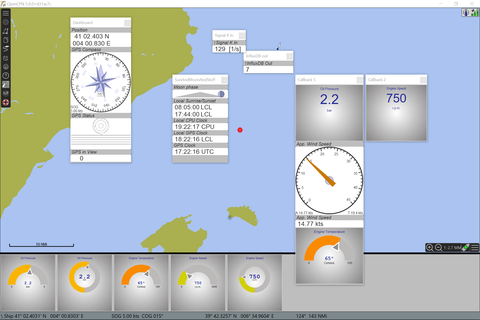
\includegraphics{2020-02-13_DashT_EngineDJG_proto_screenshot.png}
\href{img/2020-02-13_DashT_EngineDJG_proto_screenshot.png}{(zoom)}

    \hypertarget{nmea-2000-as-data-source}{%
\section{NMEA-2000 as data source}\label{nmea-2000-as-data-source}}

    NMEA-2000, a derivation of the CAN data bus is the most likely commodity
off the shelf (COTS) source for engine and energy data on boats with
recent electronics (albeit it may have a commercial name for © and ®
business reasons). Shortly, what the CAN-bus is doing in your car,
NMEA-2000 is used to the same in your boat. NMEA-0183 remains, of course
a data source for other DashT instruments but not for EngineDJG
instruments.

    \hypertarget{signal-k-as-data-interchange-protocol}{%
\section{Signal K as data interchange
protocol}\label{signal-k-as-data-interchange-protocol}}

    \href{https://opencpn.org/wiki/dokuwiki/doku.php?id=opencpn:supplementary_software:signalk}{Signal
K}, a modern and open data format for marine use is a protocol
understood by DashT for data interchange over the network.
\href{https://github.com/SignalK/specification/blob/master/gitbook-docs/keys.md}{Signal
K keys} are defined for each data source, called below \textbf{data
paths}. An EngineDJG instrument subscribes to the data coming from one
of the data path using a Signal K key.

    In order to use EngineDJG instrument in DashT, one needs therefore to
have a \emph{Signal K server node} interfacing with the boat's
instrumentation NMEA-2000 databus. It is available for
\href{https://github.com/SignalK/signalk-server-node/blob/master/raspberry_pi_installation.md}{Raspberry
PI/Linux}, for
\href{https://opencpn.org/wiki/dokuwiki/doku.php?id=opencpn:supplementary_software:signalk:a3}{Windows}
and eventually on Mac, since is based on
\href{https://nodejs.org}{node.js}. Please read more from
\textbf{\emph{O}}penCPN
\href{https://opencpn.org/wiki/dokuwiki/doku.php?id=opencpn:supplementary_software:signalk}{supplementary
software pages}.

    \hypertarget{how-it-works}{%
\subsection{How it works}\label{how-it-works}}

    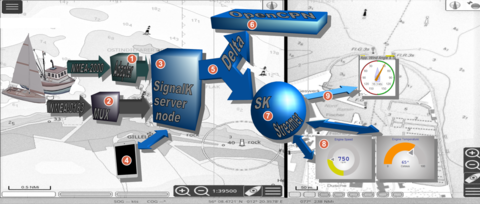
\includegraphics{2020-02-13_DashT_EngineDJG_SK_diagram_enumerated.png}
\href{img/2020-02-13_DashT_EngineDJG_SK_diagram_enumerated.png}{(zoom)}

    (\textbf{1}). NMEA-2000 databus is the source of the engine and energy
data for the EngineDJG instrument.

\begin{quote}
There may be other, potential data sources which can be enabled in the
future, such as IoT capable sensors, Bluetooth Low Energy (BLE) and
General Purpose I/O pins (GPIO) but for now, only NMEA-2000 is selected
as data source.
\end{quote}

    (\textbf{2}). In case the NMEA-2000 databus does not provide
navigational data, needed by \textbf{\emph{O}}penCPN and displayed by
other DashT instruments, your boat probably sports also a classic
NMEA-0183 wired sensors and instruments. They end up, typically into a
multiplexer (MUX), which interfaces simply with the Signal K server node
either by a USB connection, Ethernet connection or WiFi.

    (\textbf{3}). Signal K node server, or a commercial Signal K data
enabled router / multiplexer is entirely network enabled and can locate
anywhere in your boat, not necessarily on the same computer where one is
running \textbf{\emph{O}}penCPN and DashT

    \begin{quote}
Signal K data format is a standard for data interchange. A server
implements and a client uses that data format. For example ``Signal K
server node'' is not ``Signal K'', it is one of its implementations but
there are others. See
\href{https://opencpn.org/wiki/dokuwiki/doku.php?id=opencpn:supplementary_software:signalk:a2}{this
list} of open source and commercial products available.
\end{quote}

    (\textbf{4}). For example, one can have immediately access from the
cockpit table to the rich set of instruments, plug-ins and features
Signal K server node provides

    (\textbf{5}). Signal K standard defines and a server node provides,
among its other networked data interchange interfaces, so-called
Delta-channel, where all the changes in the boat data is available. When
the boat has a NMEA-2000 databus this usually means a lot of data and
many Signal K keys. Clients can subscribe to all of this data or to some
selected keys only.

    (\textbf{6}). \textbf{\emph{O}}PenCPN has developed an interface to
Signal K. Of course, it is not a consumer of engine data and it is not
even remotely interested in knowing if the ice cube machine is still
working but it needs the time, position and other navigational data for
its routing and map functions. Also, it needs to feed the majority of
its plug-ins - including DashT - with NMEA-0183 data through its
internal multiplexer gateway towards these third party consumers. Even
though the Signal K Delta channel interface would not be used in
\textbf{\emph{O}}penCPN, a Signal K server node is able to provide the
data in NMEA-0183 format to the chartplotter.

    (\textbf{7}). DashT plug-in for \textbf{\emph{O}}penCPN chartplotter
contains an efficient, built-in Signal K data streamer. It subscribes to
\emph{all} data a Signal K server sends over the Delta channel and
distributes the data to its own subscribers over a very efficient
call-back function mechanism. This way, it makes gain in speed and
lowers the number of network connections to the Signal K node server,
reducing its workload.

    (\textbf{8}). The EngineDJG instrument comes only in one flavour, unlike
other DashT's ``traditional'' Dashboard navigational instruments which
are hard-coded for their intended usage. An EngineDJG instrument is
configured after its creation. The user of the instrument is provided
with a list of available Signal K keys. Only one of the keys can be
selected per instrument. The origin of the data must be a NMEA-2000 data
source, currently. The data must be presented as a numerical value which
makes 0/1 type of status information not likely candidate to be shown
nicely on these instruments. Three possible presentations are provided,
a dial in 180 degrees, a donut in 360 degrees and a simple numerical
output. One swap between the presentation styles with Ctrl+arrowUp or
Ctrl+arrowDown keys.

    (\textbf{9}). The traditional Dashboard instruments, such as wind data
and similar are subscribed automatically to the corresponding Signal K
key. If it is not available, they will receive the data as before, from
the \textbf{\emph{O}}penCPN's NMEA-0183 distribution channel.

    \hypertarget{installation}{%
\section{Installation}\label{installation}}

    The EngineDJG gauge does not require any additional installations, all
the components are incorporated in the plug-in and ready to use.

    \hypertarget{signal-k-server-node}{%
\subsection{Signal K server node}\label{signal-k-server-node}}

    If you have already in your boat a Signal K server node running on a
computer, interfacing with and reading data from your boat's NMEA-2000
bus or from its commercial derivations, you are all set!

    In the opposite case, please read first the
\href{http://signalk.org/overview.html}{Signal K overview}. Few
implementations exists for the servers providing Signal K data. There is
an
\href{https://opencpn.org/wiki/dokuwiki/doku.php?id=opencpn:supplementary_software:signalk}{OpenCPN
supplementary software documentation page} which provides you more
information about the available servers.

    One of the server implementations providing fast and reliable networked
data in Signal K data interchange format is
\href{https://github.com/SignalK/signalk-server-node}{Signal K server
node} - please avoid the pitfall suggested by the name: ``Signal K
server node'' is not ``Signal K data format'' and vice versa but a
server implementation using that data format. The \emph{node} in Signal
K server node means that it implemented as a JavaScript server node for
\href{https://nodejs.org/en/}{Node.js} which is a ``\emph{JavaScript
runtime built on Chrome's V8 JavaScript engine}''. Both Node.js and the
Signal K server implementation are very robust and highly network
communication efficients.

    A typical configuration would take the advantage of those communication
abilities by making the Signal K server node running on the boat's
computer, which can be typically an embedded device connection to the
boat's instrumentation bus, Bluetooth or IoT devices and, why not,
running also the \textbf{\emph{O}}penCPN chartplotter - the power of the
recent embedded boards is astonishing and they come with 4K screen
support making them a perfect low-power fit for the chart table.

    Since we can communicate within a networked boat and perhaps even out of
it with alarms and such, a typical installation would consist an
external navigation computers with \textbf{\emph{O}}penCPN chartplotter
and DashT plug-in, phones and tables alike which can be taken to the
cockpit.

    Now, when you have a Signal K node server in your boat's installation
and can use, for example your tablet to connect to the Signal K server
and its built-in instrument support, you can do alike with the DashT
EngineDJG instruments and integrate the same information in the
Dashboard of the \textbf{\emph{O}}penCPN chartplotter.

    \begin{quote}
A comprehensive Developer's Guide (\href{./developers/README.html}{html}
\textbar{} \href{./developers/README.pdf}{pdf}) is provided for those
who prefer to go a different way by forking this project and adapting it
to their ideas and likings.
\end{quote}

    \hypertarget{configuration}{%
\section{Configuration}\label{configuration}}

    This chapter is addressing the first time configuration - \emph{i.e.}
the adaptation into the networked infrastructure of your boat - and the
configuration of DashT EngineDJG instruments themselves.

    \hypertarget{adaptation-into-your-boats-network-infrastructure}{%
\subsection{Adaptation into your boat's network
infrastructure}\label{adaptation-into-your-boats-network-infrastructure}}

    This part is about impossible to automate since probably only you know
where things are running in your boat! The good news is that since you
have already a Signal K server node up and running and the network
connections all set, we just need to use those connections and use their
settings!

    \hypertarget{signal-k-streamer}{%
\subsubsection{Signal K streamer}\label{signal-k-streamer}}

    Signal K streamer is used not only by DashT EngineDJG instruments,
therefore it has its own user's guide
(\href{../signalk/SignalKInputStreamerUsage.html}{html} \textbar{}
\href{../signalk/SignalKInputStreamerUsage.pdf}{pdf}). Make it work
first, otherwise no data will flow in.

    \hypertarget{making-dasht-enginedjg-instruments-available-on-network}{%
\subsubsection{Making DashT EngineDJG instruments available on
network}\label{making-dasht-enginedjg-instruments-available-on-network}}

    The instrument is composed of a HTML file and numerous JavaScript files,
like any other browser based application. The configuration task consist
of making them available on your boat's network. It contains many
elements being platform specific, explained in below sections.

    \begin{quote}
NOTE: one may be tempted to use \emph{file://} protocol. Please note
that in Windows, starting from
\href{https://support.microsoft.com/en-us/help/4534251/cumulative-security-update-for-internet-explorer}{security
update of 2020-01-14} local storage capability, including cookies is
disabled for \emph{file://} protocol in the back-end the wxWidgets is
using on Windows (IE). Therefore we address below only the usage of
\emph{http://} protocol to retrieve files from your files infrastructure
to enable persistent EngineDJG configuration settings across platforms.
\end{quote}

    \hypertarget{dasht-enginedjg-publishing-on-linux}{%
\paragraph{DashT EngineDJG publishing on
Linux}\label{dasht-enginedjg-publishing-on-linux}}

    First, you have to identify where are the DashT EngineDJG files after
the installation and export the directory:

    \texttt{/usr/share/opencpn/plugins/dashboard\_tactics\_pi/data/instrujs/}

    \hypertarget{apache2-server}{%
\subparagraph{Apache2 server}\label{apache2-server}}

    Most of the Linux systems provide Apache2 server by default and even
start it by default. Navigate to your Linux box's network IP-address and
you will soon find out if this is the case. Otherwise, it is not a big
task to get it running but for clarity we presume now that it is already
active. You would say:

    \texttt{sudo\ ln\ -s\ /usr/share/opencpn/plugins/dashboard\_tactics\_pi/data/instrujs\ /var/www/html/instrujs}

    Check that it works (here the IP-address is an example only, use your
own):

    \begin{figure}
\centering
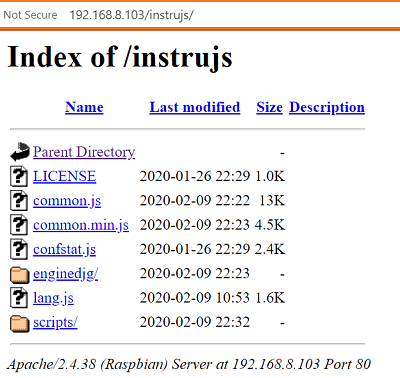
\includegraphics{2020-02-15_Apache2_check_instrujs.png}
\caption{2020-02-15\_Apache2\_check\_instrujs.png}
\end{figure}

    \hypertarget{http-server-node}{%
\subparagraph{http-server node}\label{http-server-node}}

    Since you already have a Signal K server node you have thus
\emph{node.js}. If the above Apache2 method seems like an overkill to
you, there is this dead simple solution:

    \texttt{npm\ install\ -g\ http-server}

    If you take a look at the DashT distribution directory above, you will
find a shell script \texttt{httpserver.sh}. It contains simply:

    \begin{verbatim}
#!/usr/bin/env bash
http-server /usr/share/opencpn/plugins/dashboard_tactics_pi/data/instrujs/ -p 8088
\end{verbatim}

    Execute the script, leave the http-server running and verify that files
are available on the port \texttt{8088} (you can modify the port, of
course):

    \begin{verbatim}
pi@pi:~/dev/dashboard_tactics_pi/data/instrujs/scripts $ ./httpserver.sh 
Starting up http-server, serving /usr/share/opencpn/plugins/dashboard_tactics_pi/data/instrujs/
Available on:
  http://127.0.0.1:8088
  http://192.168.8.103:8088
Hit CTRL-C to stop the server
\end{verbatim}

    \begin{figure}
\centering
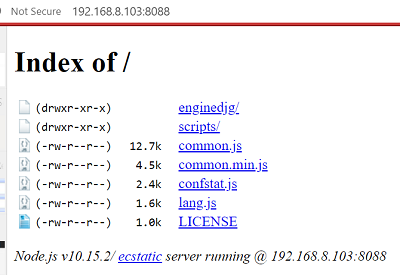
\includegraphics{2020-02-15_Ecstatic_check_instrujs.png}
\caption{2020-02-15\_Ecstatic\_check\_instrujs.png}
\end{figure}

    \hypertarget{dasht-enginedjg-publishing-on-windows}{%
\paragraph{DashT EngineDJG publishing on
Windows}\label{dasht-enginedjg-publishing-on-windows}}

    \begin{quote}
We suppose below that you are running also the Signal K server node on
Windows. Otherwise, please refer to above instructions on Linux to
publish DashT EngineDJG files on your boat's network infrastructure.
\end{quote}

    In addition to the Signal K server node
Section \ref{signal-k-server-node}, install also the following server
node:

    \texttt{npm\ install\ -g\ http-server}

    You will find the files to share from
\texttt{C:\textbackslash{}Program\ Files\ (x86)\textbackslash{}OpenCPN\textbackslash{}plugins\textbackslash{}dashboard\_tactics\_pi\textbackslash{}data\textbackslash{}instrujs}

    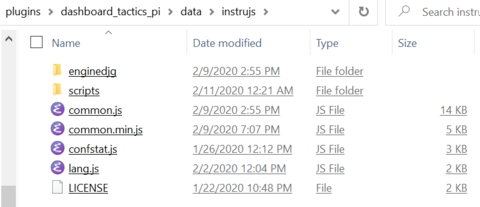
\includegraphics{2020-02-15_Windows_Explorer_instrujs_dir.png}
\href{img/2020-02-15_Windows_Explorer_instrujs_dir.png}{(zoom)}

    Move to the \texttt{scripts}folder.

    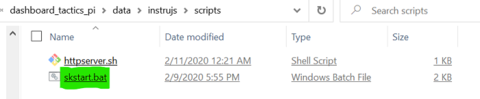
\includegraphics{2020-02-15_Windows_Explorer_scripts_dir.png}
\href{img/2020-02-15_Windows_Explorer_scripts_dir.png}{(zoom)}

    Copy the file on your desktop. Observe the file's contents, these lines:

    \begin{verbatim}
start signalk-server
start http-server
\end{verbatim}

    You can see that the batch file starts both the Signal K server node and
HTTP server node and launches the Signal K server node's graphical user
interface on your default browser. Using that browser, open a new window
or tab and check that the DashT EngineDJG files are also available:

    \begin{figure}
\centering
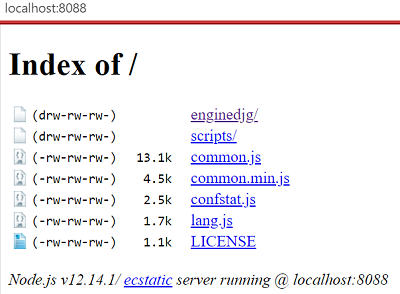
\includegraphics{2020-02-15_Ecsatic_check_instrujs_localhost_windows.png}
\caption{2020-02-15\_Ecsatic\_check\_instrujs\_localhost\_windows.png}
\end{figure}

    \hypertarget{tell-dasht-where-to-find-enginedjg-files}{%
\subsubsection{Tell DashT where to find EngineDJG
files}\label{tell-dasht-where-to-find-enginedjg-files}}

    Now that you have set your network infrastructure and know exactly where
the EngineDJG files need to be loaded from, you need to set that URL
into the \textbf{\emph{O}}penCPN configuration file.

    The easiest way to do this is to configure one DashT EngineDJG
instrument
(Section \ref{adding-and-configuring-dasht-enginedjg-instruments}) and
ignore the probable fact that the loading of the EngineDJG files will
fail with the default settings: just quit the \textbf{\emph{O}}penCPN.
This will create an entry in the \emph{opencpn.ini} (or
\emph{opencpn.conf} on Linux) which you can edit. Here we set it with
the above example on Windows, to be retrieved from the local host:

    \begin{verbatim}
[PlugIns/Dashboard/WebView]
[PlugIns/Dashboard/WebView/EngineDJG]
instrujsURL=http://localhost:8088/enginedjg/
\end{verbatim}

    \hypertarget{configuration-of-dasht-enginedjg-instruments}{%
\subsection{Configuration of DashT EngineDJG
instruments}\label{configuration-of-dasht-enginedjg-instruments}}

    \begin{quote}
NOTE: Configuration can take place only when the instruments receive
data from the Section \ref{signal-k-streamer}
\end{quote}

    \hypertarget{adding-enginedjg-instruments}{%
\subsubsection{Adding EngineDJG
instruments}\label{adding-enginedjg-instruments}}

    EngineDJG instruments are compatible with all Dashboard instruments and
they can be added in any Dashboard instrument cluster window pane.
However, since the number of engine parameters, for example is important
it is suggested that you create instruments clusters like for ``Engine''
data and for ``Energy'' data.

    The adding of instruments is like adding any other Dashboard instrument
in DashT's preferences: scroll all the way down of the list to find the
single instrument. Add as many instances of it as you estimate you are
going to need to show the data parameters you are interested in.

    It is suggested than before the configuration the instrument cluster is
in ``Horizontal'' mode to allow sometime very long menu list presented
during the configuration phase to roll out vertically. Once the
instrument cluster window pane is configured, one can change, of course
to ``Vertical'' mode if needed.

    \begin{figure}
\centering
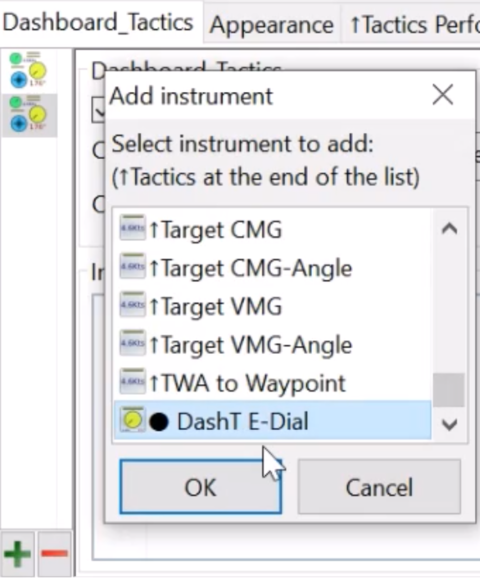
\includegraphics{2020-02-15_Adding_DashT_EngineDDG-1.png}
\caption{2020-02-15\_Adding\_DashT\_EngineDDG-1.png}
\end{figure}

    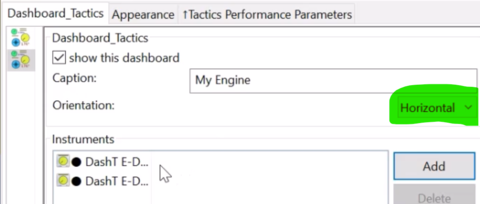
\includegraphics{2020-02-15_Adding_DashT_EngineDDG-2.png}
\href{img/2020-02-15_Adding_DashT_EngineDDG-2.png}{(zoom)}

    How-to video: ()

    \hypertarget{subscribing-enginedjg-instruments-to-data-paths}{%
\subsubsection{Subscribing EngineDJG instruments to data
paths}\label{subscribing-enginedjg-instruments-to-data-paths}}

    Once a new DashT EngineDJG instrument has been created it asks from
DashT's Signal K streamer what available data paths there are. It
requires a complete list and, depending of your boat's instrumentation
this can be a pretty long list. Normally it should be finished in less
than 10 seconds, though.

    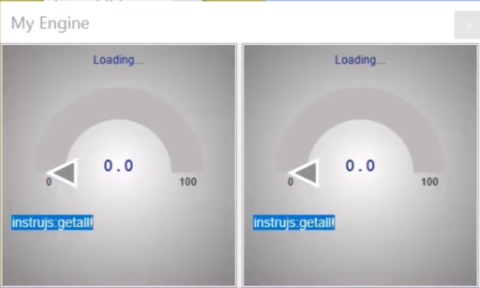
\includegraphics{2020-02-15_EngineDJG_loading_all_paths.png}
\href{img/2020-02-15_EngineDJG_loading_all_paths.png}{(zoom)}

    Once a list of all available data paths has been received, DashT
EngineDJG instrument builds a selection menu out of them and invites you
to make your selection using the context menu which is activated by a
maintained right click on the upper left hand corner of the instrument.

    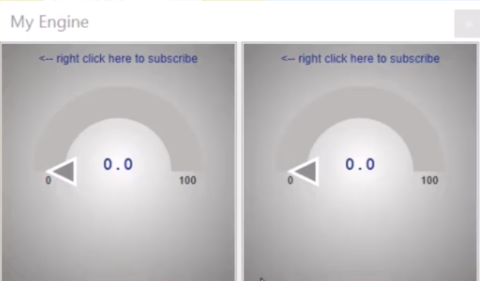
\includegraphics{2020-02-15_EngineDJG_received_all_paths.png}
\href{img/2020-02-15_EngineDJG_received_all_paths.png}{(zoom)}

    In the context menu, all available data paths are listed a hierarchical
order. The names of the data paths are usually clear enough to
understand the nature and the origin of the data. A full list of
\href{https://github.com/SignalK/specification/blob/master/gitbook-docs/keys.md}{Signal
K keys} is also available.

    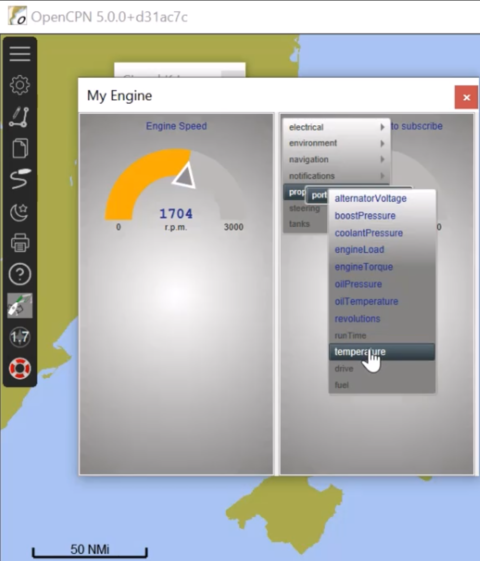
\includegraphics{2020-02-15_EngineDJG_select_from_available_paths-1.png}
\href{img/2020-02-15_EngineDJG_select_from_available_paths-1.png}{(zoom)}

    The data path values where the last element is marked in blue means that
the DashT installation package has a pre-defined setting for it and it
can be shown by simply selecting that data path.

    \begin{figure}
\centering
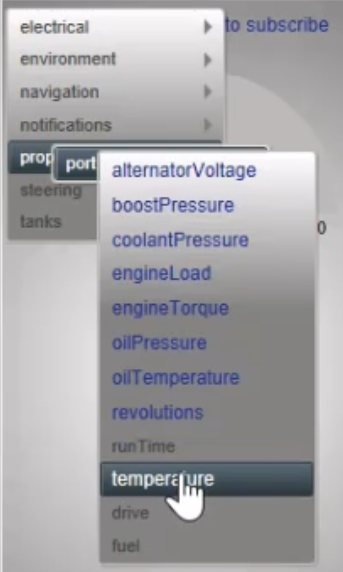
\includegraphics{2020-02-15_EngineDJG_select_from_available_paths-2.png}
\caption{2020-02-15\_EngineDJG\_select\_from\_available\_paths-2.png}
\end{figure}

    Most common data path values have been included in the DashT
installation by default for engine and some most obvious data paths for
the energy. If the data path is grayed out, it means that it cannot be
selected since no data path rule has been defined. This does not mean
that the value cannot be shown, it is just that the development and
testing has not been able to test it or are not aware of it - there is
really a lot of data paths of all sort, such as status data. A way to
define your own configuration for data paths is discussed
Section \ref{adding-new-data-paths-of-your-own}.

    \hypertarget{search-again-for-the-available-data-paths}{%
\paragraph{Search again for the available data
paths}\label{search-again-for-the-available-data-paths}}

    If you cannot find a data path you are expecting to find from the menu,
you can ask for a quick rescan by selecting any of the grayed-out items
from the menu, \emph{i.e.} a menu item which is not in blue color. You
may get an alert of a non-existing path, depending of the common
configuration file settings. Resulting action is, anyway the same as in
Section \ref{changing-enginedjg-instruments-data-path-subscription} and
the data sources are scanned again for new paths.

    \begin{quote}
NOTE: The available data scanning is cumulative and if the data path you
are expecting was not available from your data bus within the previous
scan's time window frame (in less than 10 seconds), it may have been
omitted. Rescan may help. Once the path is recongnized and configured,
the subsription to it will be persistent.
\end{quote}

    \hypertarget{select-different-display-type}{%
\paragraph{Select different display
type}\label{select-different-display-type}}

    You can scroll the display types with Ctrl+\(\uparrow\) and
Ctrl+\(\downarrow\) (Ctrl-key kept down and press arrow keys up or
down): apart the default 180-degree dial type, there is also a
360-degree `donut' and a simple numerical display type available.

    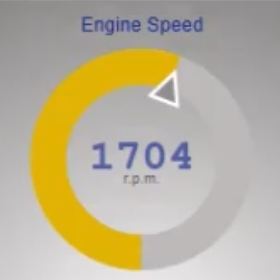
\includegraphics{2020-02-15_EngineDJG_display_donut.png} \textbar{}
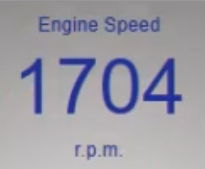
\includegraphics{2020-02-15_EngineDJG_display_simple.png}

    How-to video: ()

    \hypertarget{changing-enginedjg-instruments-data-path-subscription}{%
\subsubsection{Changing EngineDJG instrument's data path
subscription}\label{changing-enginedjg-instruments-data-path-subscription}}

    While the EngineDJG is running (\emph{i.e.} data is coming in by an
existing subscription a data path from the Signal K streamer)
right-click on the upper left corner in order to get the context menu
which allows you to stop the data display and force a complete
re-initialization of the data path subscription as explained in the
previous section.

    How-to video: ()

    \hypertarget{customization}{%
\subsection{Customization}\label{customization}}

    It goes without saying that nobody else but \textbf{you} will be able to
find out the particular data sources available in your own boat! DashT
EngineDJG reports you all the data paths but the distribution makes a
modest guess what might interest you in the first place. It is likely
that we miss something.

    Unlike the rest of the DashT, which is written in C++/wxWidgets, the
EngineDJG is a JavaScript program which means there are plain text files
which you can modify, allowing you to customize the data paths displayed
according to your requirements.

    Modern web development techniques have been used which result in a very
compact and thus non-human readable run-time program execution format,
but two files are provided in plain text without compression which
allows you to make your own customizations.

    In above chapters you defined
Section \ref{making-dasht-enginedjg-instruments-available-on-network} in
your boat's network and computer infrastructure.

    \begin{quote}
NOTE: Make sure to take backups before modifying anything!
\end{quote}

    \hypertarget{adding-new-data-paths-of-your-own}{%
\subsubsection{Adding new data paths of your
own}\label{adding-new-data-paths-of-your-own}}

    You would need to modify a configuration file named \texttt{common.js} -
here is an excerpt of the instructions in that file

    \begin{verbatim}
 Contribute/report here, please:
\end{verbatim}

\begin{quote}
https://git.io/JejKQ
\end{quote}

\begin{verbatim}
 - with a screenshot and a short description of your installation, thanks!
 SignalK Path keys:
\end{verbatim}

\begin{quote}
https://git.io/JvsYw
\end{quote}

\begin{verbatim}
 The Signal K values are always in SI units (like m/s, not knots).
 Conversion to a wanted unit is made with multipier/division/offset.
 Avoid using floating point values like 0.000000003 in JavaScript!
 UTF8 - do _not_ change encoding, cf. degree character. Notepad++ recommended.
 Usage example: enginedjg/index.html loads a minimized version, common.min.js
        - make a copy of common.min.js by renaming it;
        - make a copy of this one with name common.min.js and modify it;
        - (no need for compression with this non-executing file!)
        - or, modify enginedjg/index.html to load your own file, no problem!
        - issues? open the index.html in a browser, hit Shift+Ctrl+I and reload;
                  * Console gives you the reason why it does not load anymore:
                  * Look for messages in red, a typo, missing comma?
        - note: next update/reinstallation overrides this file, keep backups!
\end{verbatim}

    Typical change that you may want to do is to have different titles for
each battery parks, instead of having a \texttt{*} wild card. You would
copy-paste-modify the below definition with a wild card to individual,
full data path (Signal K key) name and a title for your liking as many
times your system is reporting about them:

    \begin{verbatim}
        {
            version    : 1,
            path       : 'electrical.batteries.*.current',
            title      : 'Battery Current',
            symbol     : '',
            unit       : 'Amps',
            display    : 'dial',
            decimals   : 1,
            minval     : -20,
            loalert    : 0,
            hialert    : 0,
            maxval     : 20,
            multiplier : 1,
            divider    : 1,
            offset     : 0
        },
\end{verbatim}

    Of course, you may want to simply change units in some entries, like
from Celsius to Fahrenheit. Just be careful to preserve the UTF-8 degree
sign, will you.

    The header part of the file contains some common customizations, like
turning off the alerts or giving more time for them to set in. One can
also increase the debug level in case the EngineDJG HTML/JS code needs
to be inspected in an external browser. Please note the above: the file
is \textbf{not} used by default but one needs to replace the compressed
version of it with this human readable one. Follow the instructions for
that. If a need arise, do not hesitate to do that - there is no
performance penalty since the file is read only during the startup of
instruments.

    \hypertarget{make-enginedjg-talking-your-language}{%
\subsubsection{Make EngineDJG talking your
language}\label{make-enginedjg-talking-your-language}}

    Unfortunately, it is self service, no community support. Yet! You can
participate with your native tongue by submitting your translations
here: https://git.io/JejKQ

    Meanwhile, you can just replace the \texttt{lang.js} file with yours.
Keep a copy of the original, though: JavaScript does not make any gifts
but goes to a grinding halt for any syntax error and none of the DashT
EngineDJG instruments will start!

    \hypertarget{troubleshooting}{%
\section{Troubleshooting}\label{troubleshooting}}

    \hypertarget{data-does-not-look-right-to-me}{%
\subsection{Data does not look right to
me}\label{data-does-not-look-right-to-me}}

    It is always a good idea to go back as close as possible to the data
source, which is Signal K server node. What does it say about that data?
If the SI unit value it displays in its own plug-ins and log files makes
sense to you, then the issue is probably with the multiplier, divider or
offset, or all of them used to convert it (see above sections about the
customization). The floating point data which is coming from Signal K
server node is given as such to DashT EngineDJG instrument, but as a
string (we are talking to a JavaScript program) in scientific notation
with single decimal format. For example, if DashT receives 0.24444444,
it will be given as ``24.5E-2'' to EngineDJG instrument. General rule is
that values with too many zeros are not advisable in JavaScript. Avoid
calculations where any result, including intermediate values would lead
to values like 0.0000003.

    If things need deep understanding of data which is coming in from your
boat's databus, maybe the easiest place where you can look at it is the
log files of Signal K server node's databus connector. You need to
activate them explicilty. Developer's Guide
(\href{./developers/README.html}{html} \textbar{}
\href{./developers/README.pdf}{pdf}) provides some use cases of deep
packet analysis but be warned, it is not for faint hearted!

    \hypertarget{i-edited-a-file-and-all-dasht-enginedjg-instruments-are-now-dead}{%
\subsection{I edited a file and all DashT EngineDJG instruments are now
dead!}\label{i-edited-a-file-and-all-dasht-enginedjg-instruments-are-now-dead}}

    The good and bad of JavaScript is that as a scripted language it allows
you to make as many syntax errors you like. When you are editing, that
is\ldots{} Since there is no compilation the eventual errors are
detected only during loading and even worse, sometimes during the
run-time when the code execution passes in the faulty section!

    Your best friend is your ordinary browser. Point it to the data
directory where the EngineDJG \texttt{index.html} file is located and
see if you can see an empty dial. If you do not see, then hit
\texttt{Shift+Ctrl+I} (Shift and Ctrl-keys hold down and press key
``I'') to open the developer tools. Select the Console and hit F5 to
reload the page. Usually, the point where the syntax error is located is
clearly shown in red color.

    \begin{quote}
Windows owners should not throw away their beloved (?) Internet Exlorer.
In fact, the wxWidgets WebView back-end is as old as IE8! In that case,
having the IE11 is not a bad idea for testing: you would hit key F12 to
get the developer tools visible in this case.
\end{quote}


    % Add a bibliography block to the postdoc
    
    
    
\end{document}
